\chapter{Discussion}
In the present chapter, the previously described results are analyzed in detail and further discussed following the same order as in the previous chapter: starting with the base simulation results and following with the size and volatile content variability. Then, the implications for the IDDP-1, and potentially other shallow magma pockets, are addressed.

\section{Results analysis}
%\subsection{Temperature}
Starting with the temperature results, the most impactful and obvious feature is the quasi-stall cooling trend that develops after approximately 50 years of simulated time when the averaged (or integrated) temperature cools down to approximately 830°C. At this temperature, the volume fraction of crystals, following the crystallization curve in figure \ref{fig:vfc_vs_temp}a is around 0.01, which results in an extremely low number. However, the temperature plot shows the integrated temperature of the whole magma, which means that the temperature is not uniform. There are some areas with higher temperature, and areas where temperature is low enough to crystallize further. In particular, an as it shown in figure \ref{fig:vfc_vs_temp}b, the minimum temperature in this simulations is 774.5°C, which is low enough to crystallize ~0.32 volume fraction. The formation these batches, and a total volume fraction of crystals of ~0.06 (which can be considered the critical crystallinity) in the interior of the magma can be described at the onset of the stepped cooling behavior, since the release of heat due to crystallization (latent heat of phase change) is able to partially compensate the heat lost across the walls. This phenomena, dramatically increases the lifespan of the magma chamber. The effect of the latent heat release is present inn all the simulations, although its impact on the cooling curve differs depending on the size of the magmatic body. In the case of the \textit{large} body (red curve in figure \ref{fig:3_size_T}), the curve is apparently smooth, with little oscillations, although still present. The sharpness of the cooling-heating cycles, however, increases with reducing size. The blue curve corresponds with the smallest size, and it is clear that the oscillations are sharper than the other two, giving the curve a characteristic serrated aspect. It is also clear that the transition from smooth, continuous cooling is sudden in the \textit{small} body, occurring at exactly 20 years at 832.16 °C. This is not the case of the \textit{medium} and \textit{large}, where the transition is smooth, making it difficult to ascertain a certain point to mark the onset of the latent heat induced behavior. However, and for the sake of practicality, this point is designated at 58 years and 829.42 °C for the \textit{medium} body, and at 51 years and 829.27 °C for the \textit{large} body, corresponding to the subjective onset of curve horizontality. The difference in the sharpness of the stepped cooling behavior is a consequence of the volume of magma that is being cooled: the \textit{small} body has a large surface area-to-volume ratio. Since the cooling and the development of crystals occur from the boundaries inwards, the relative proportion of the cooling front to the volume of magma is larger, hence the relative energy released due to crystallization is proportionally larger. The \textit{large} body, acting as the direct opposite extreme to the \textit{small} body, shows the smoothest of the stepped cooling curves, and since its surface area-to-volume ratio is smaller, it is safe to assume that a larger volume of magma (an larger amount of stored enthalpy) is able to attenuate the effect of the local releases of heat due to mineral formation. Following this reasoning, a reduction in body size, and the consequent increase in surface area-to-volume ratio, would be expected to enhance the heat loss through the boundary and thereby accelerate the cooling process. As it was made obvious in \ref{fig:3_size_T}, this is only partially true, since at the early stages of the cooling process, the \textit{large} body described a more rapid cooling than the other two bodies, followed in time by the \textit{small} body. This resulted in the \textit{medium} sized body being the slowest to cool down initially. It becomes evident then that the cooling of magmatic bodies is a strongly non-linear process, where the interplay of diverse mechanisms makes it extremely difficult to predict the evolution of magmatic systems. Other mechanism introduced in these simulations, and one of the main aims of this project, is the dynamics of the magma. 

\begin{figure}
	\centering
	\begin{tikzpicture}
		\node[inner sep=0pt] (img1) at (0,0) {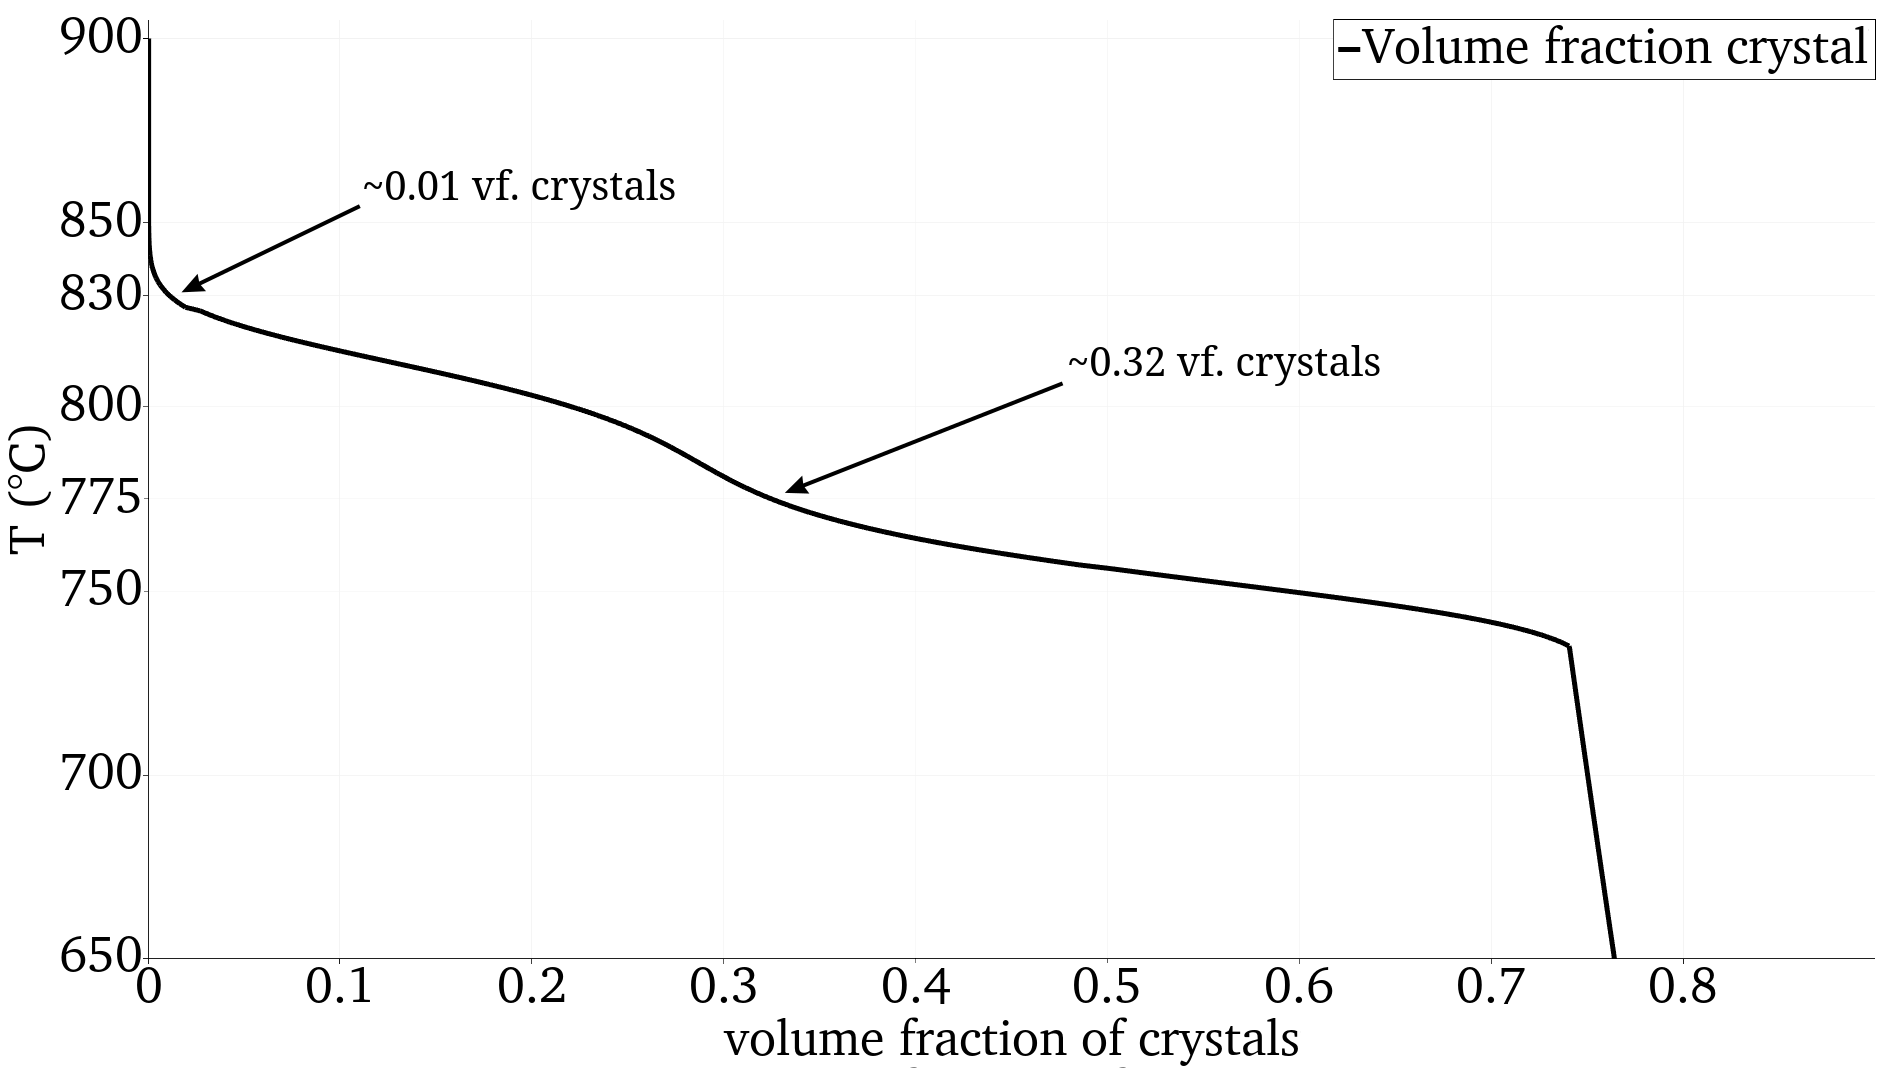
\includegraphics[width=1\linewidth]{img/chapter4/vfc_vs_T_annoted.png}};
		\node[anchor=north east, xshift=-0pt, yshift=-50pt] at (img1.north east) {\textbf{(a)}};
	\end{tikzpicture}
	\begin{tikzpicture}
		\node[inner sep=0pt] (img1) at (0,0) {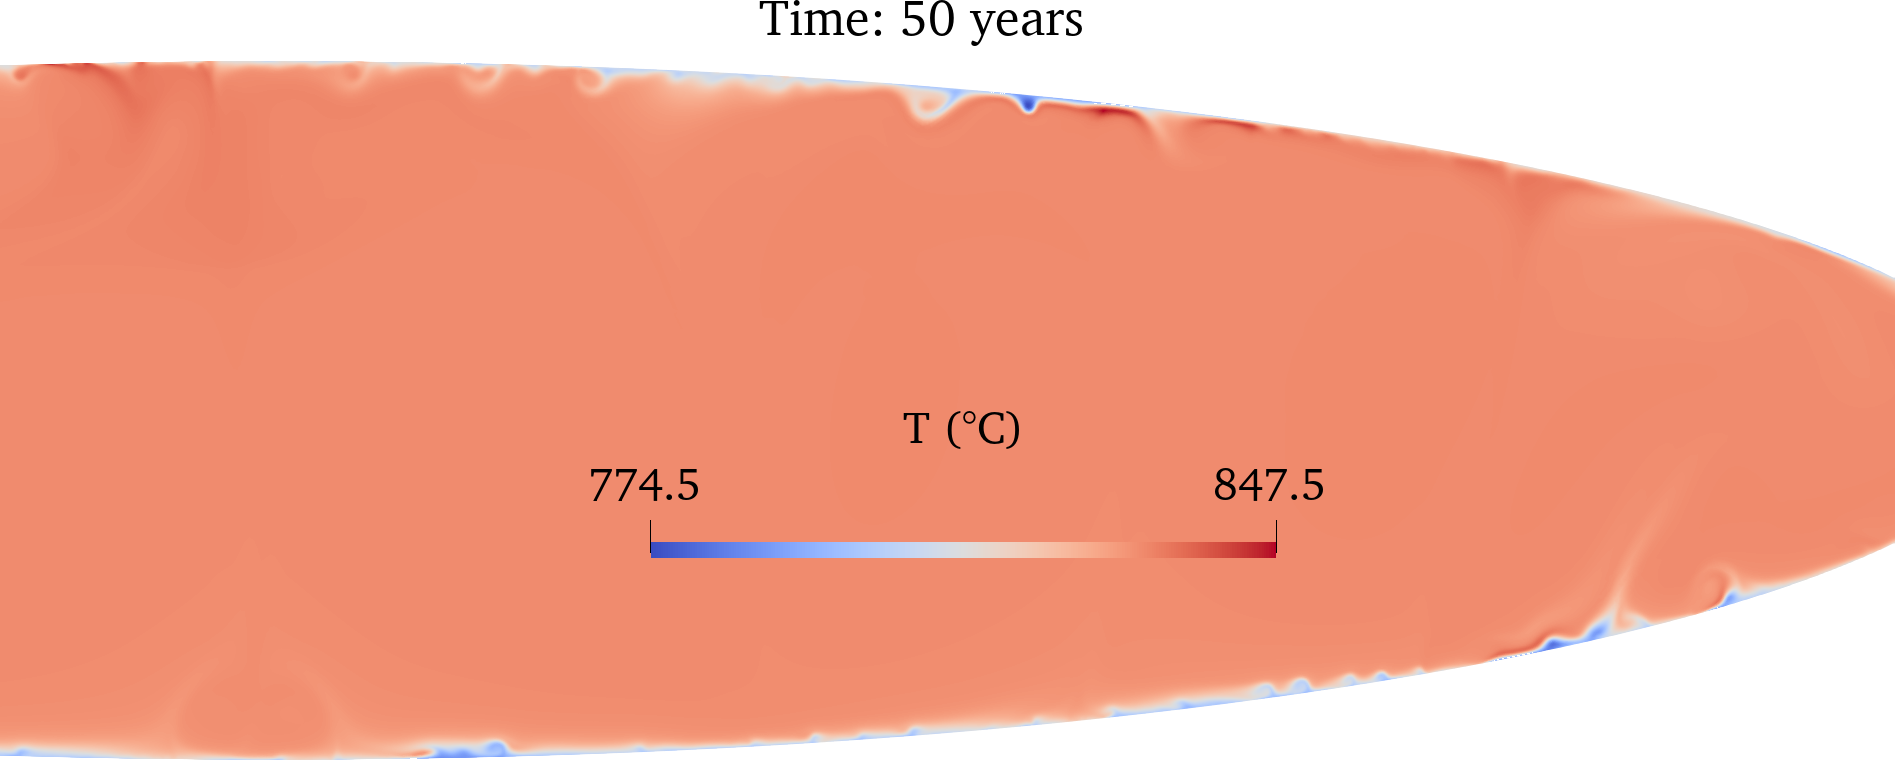
\includegraphics[width=1\linewidth]{img/chapter4/50_detail.png}};
		\node[anchor=north east, xshift=-0pt, yshift=-1pt] at (img1.north east) {\textbf{(b)}};
	\end{tikzpicture}
	\caption{a) crystal volume fraction plotted against temperature. b) snapshot of the simulation at 50 years, where some batches of cooler (hence, more crystallized) magma appear.}
	\label{fig:vfc_vs_temp}
\end{figure}

%\subsection{Velocity}
As it has being made present in the previous chapter, convection velocities vary noticeably between simulations, specially at the early stages of the simulation (see \ref{fig:3_size_v}). The maximum and averaged velocity of the \textit{large} body are higher than the other two, with values an order of magnitude faster: 2·10$^{-2}$ m/s against 5·10$^{-3}$ m/s of the \textit{medium} and 10$^{-3}$ m/s for the \textit{small}. Since velocity appears in the advection term of the heat transfer equation, the faster convection the is allowed to develop in the \textit{large} body could partially explain the faster cooling at the beginning of the simulations. However, this does not apply to the \textit{medium} body, since it is the slowest one to cool down, and the last one to reach the stepped cooling state. In this case, the balance between the heat lost trough the chamber walls, the higher enthalpy due to a more volumetric body and the velocity of the convective cells allows for a slower cooling in comparison with the other two simulation. This, once again highlights the nonlinearity of the process, which presents no clear answers to which mechanism is more important during the cooling process. 

In the case of the higher initial pressure simulation, the cooling follows practically the same curve as the base simulation until the curves diverge when the onset of the stepped cooling of the base simulation is reached. Opposite to it, the higher pressure simulation does not start to crystallize extensively and continues cooling for some more years, reaching the stepped cooling behavior at a lower temperature. This is the effect of a decrease in the liquidus temperature. Normally, an increase in pressure favors atom packing, thereby enhancing crystallization. However, the increase in pressure also favors gas dissolution, which, contrarily, inhibits crystal formation. As the main driver of crystal formation in wet magmas is volatiles exsolution, especially $H_2O$, from the melt phase, overpressure leads to a liquidus temperature decrease, hence, maintaining the magma molten at lower temperatures thought time.

The volatile content is another strong controller of the cooling and crystallization process. As it was already been shown in the precedent chapter (see \ref{fig:gas_temperature}), higher or lower gas content modify the cooling curving slope, which can delay or anticipate the onset of the stepped cooling behavior. Lower gas content (see pink curve in figure \ref{fig:gas_temperature}) plays a similar effect as the overpressure case previously discussed: since most of the less abundant gas is dissolved in the melt, mineral formation is partially inhibited. Similar behavior should be expected from the higher gas content case (see \ref{fig:gas_temperature}, yellow curve), since higher concentration of volatiles would mean more volatiles dissolved. However, in these simulations, one the amount of volatiles is increased, it's not only the $H_2O$, but also $CO_2$. Carbon dioxide strongly inhibits water activity in the melt, which necessarily means a a rise of the liquidus temperature. The effect of adding $CO_2$ to the mixture is similar to either increasing the pressure of a completely dry system, or decreasing the pressure in a wet system, forcing volatile exsolution from the melt. The initial cooling of these three cases is also different, being the faster to cool down the high volatile content magma, followed by the base simulation and the low volatile content magma. This could also be a velocity of convection effect, given that the volatile rich magma reaches higher velocities, while the volatile depleted magma is the slowest among the three (see \ref{fig:gas_velocities}). These simulations confirm that, for magmatic bodies of identical dimensions, higher convective velocities enhance the efficiency of heat transport relative to slower-moving magmas, thereby exerting an important control on the cooling of such systems. 

%\subsection{Pressure}
Pressure is characterized by an initial general decompression of the magmatic chamber in every one of the simulated bodies, with the exception of the one with low content in gas (see figures \ref{fig:3_size_dp} and \ref{fig:gas_dp}), which is due to the equilibration of the initial volatile partition, with a general dissolution of gas in the melt phase (see figure \ref{fig:integrated_vf_g}). Exsolved gas often increases the local pressure due to the low density of the phase, thus, its dissolution normally entails a decrease in pressure. This depressurization is characterized by an inversion on the difference in pressure distribution: at the start of the simulation, the top half of the simulation is being over-pressurized due to the higher presence of gas. When gas dissolution happens, accompanied by the start of convection, which sinks and drags the magma downwards, the overpressure distribution changes and undergoes an inversion, after which the bottom half of the chamber presents a positive difference in pressure, while the top half is getting depressurized. Differences on pressure, and pressure changes, are a product of density variations within the magma chamber. Crystal formation and gas exsolution locally modify the bulk density of the system, often increasing it with respect to the completely molten phase, but, on occasions, reducing it instead. This depends upon the proportion of gas with respect to crystals, since gas normally exerts a strong control over the bulk density. Figure \ref{} shows two snapshots of the base simulation: pressure difference on the top image and density on the bottom one. Higher density regions formed on the boundary, where some crystallization is taking place sink down and create regions of depressurization. This is essentially the main engine of convection.


\begin{figure}
	\centering
	\begin{tikzpicture}
		\node[inner sep=0pt] (img1) at (0,0) {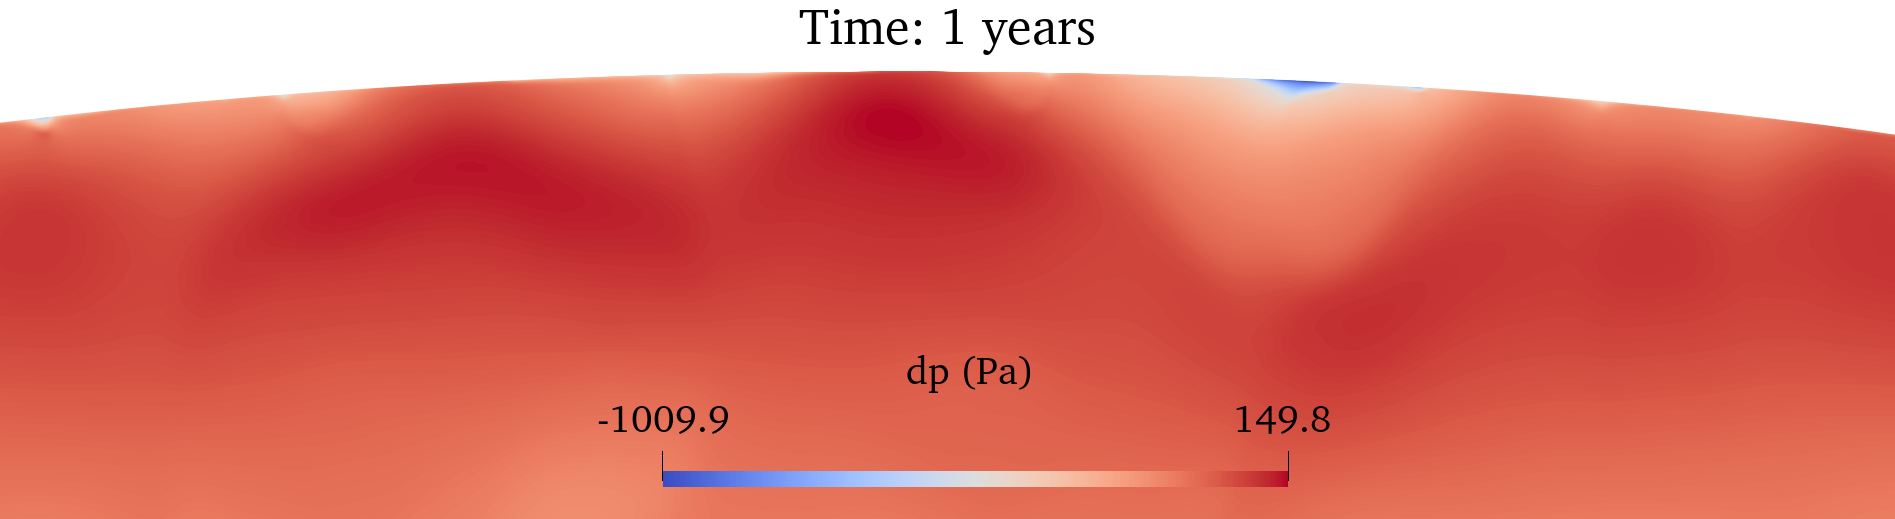
\includegraphics[width=1\linewidth]{img/chapter4/dp_rho_1.png}};
		\node[anchor=north east, xshift=-0pt, yshift=-50pt] at (img1.north east) {\textbf{(a)}};
	\end{tikzpicture}
	\begin{tikzpicture}
		\node[inner sep=0pt] (img1) at (0,0)    {
\includegraphics[width=1\linewidth]{img/chapter4/dp_rho_2.png}};
		\node[anchor=north east, xshift=-0pt, yshift=-1pt] at (img1.north east) {\textbf{(b)}};
	\end{tikzpicture}	
	\caption{Snapshots of a zoomed-in area on the base simulation comparing the pressure difference ($dp$) on top with the bulk density of the system, in the bottom image. Sinking areas of higher density material develop depressurization in them, developing convection.}
	\label{fig:dp_vs_rho}
\end{figure}


\begin{figure}
	\centering
	\begin{tikzpicture}
		\node[inner sep=0pt] (img1) at (0,0) {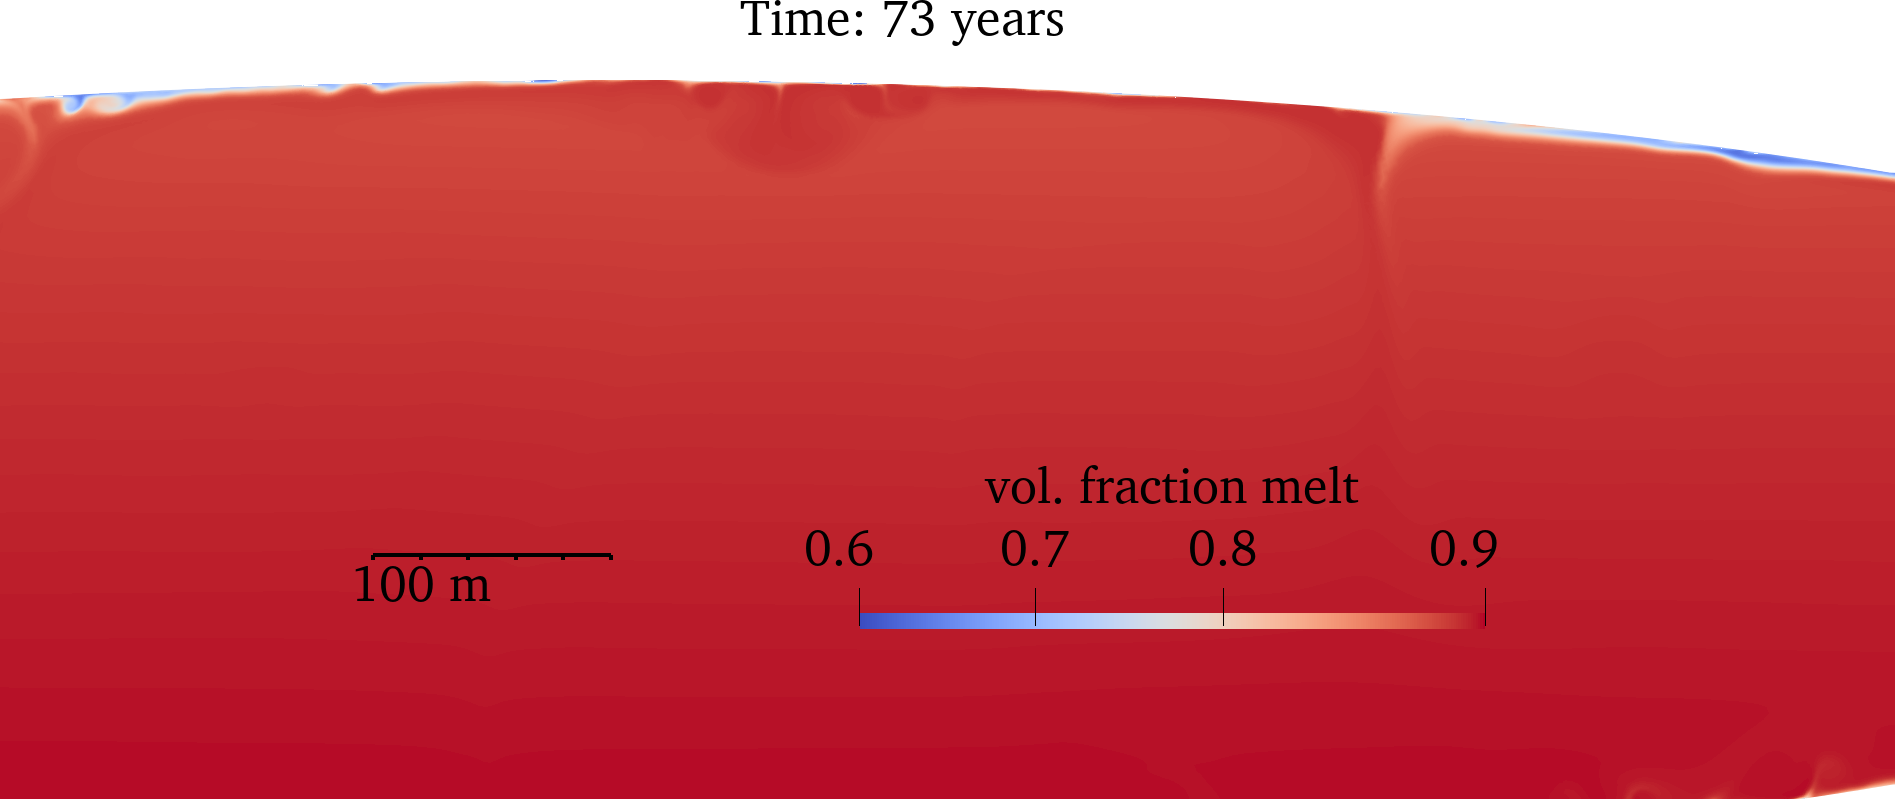
\includegraphics[width=0.86\linewidth]{img/chapter4/vf_l_73.png}};
		\node[anchor=north east, xshift=-0pt, yshift=-50pt] at (img1.north east) {\textbf{(a)}};
	\end{tikzpicture}
	\begin{tikzpicture}
		\node[inner sep=0pt] (img1) at (0,0) {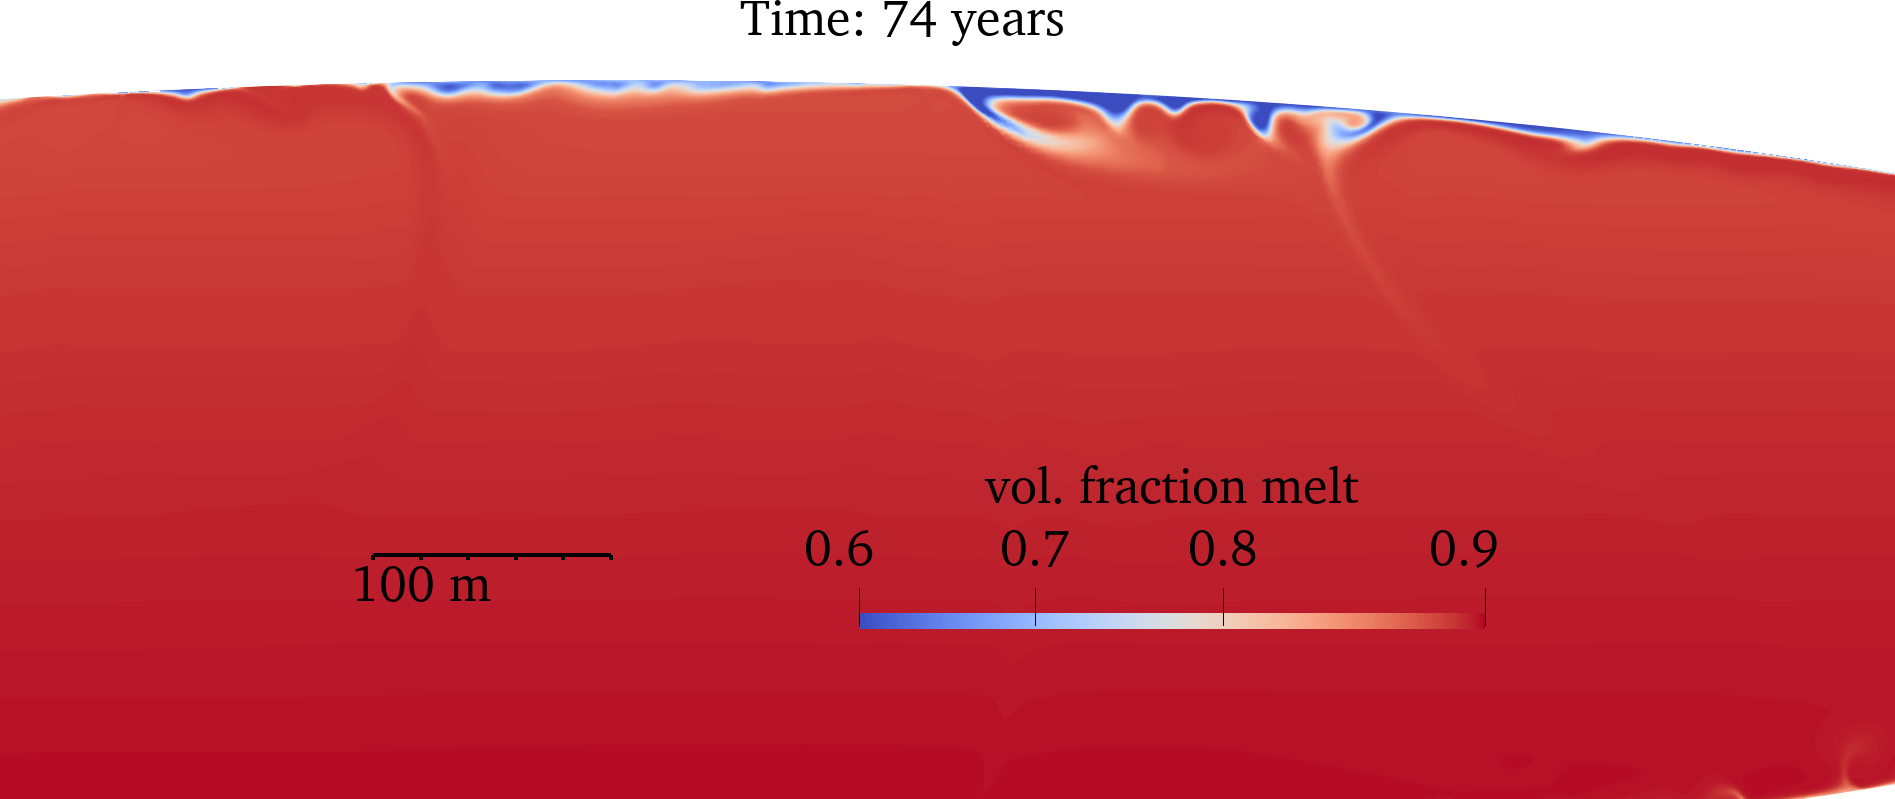
\includegraphics[width=0.86\linewidth]{img/chapter4/vf_l_74.png}};
		\node[anchor=north east, xshift=-0pt, yshift=-1pt] at (img1.north east) {\textbf{(b)}};
	\end{tikzpicture}
	\begin{tikzpicture}
		\node[inner sep=0pt] (img1) at (0,0) {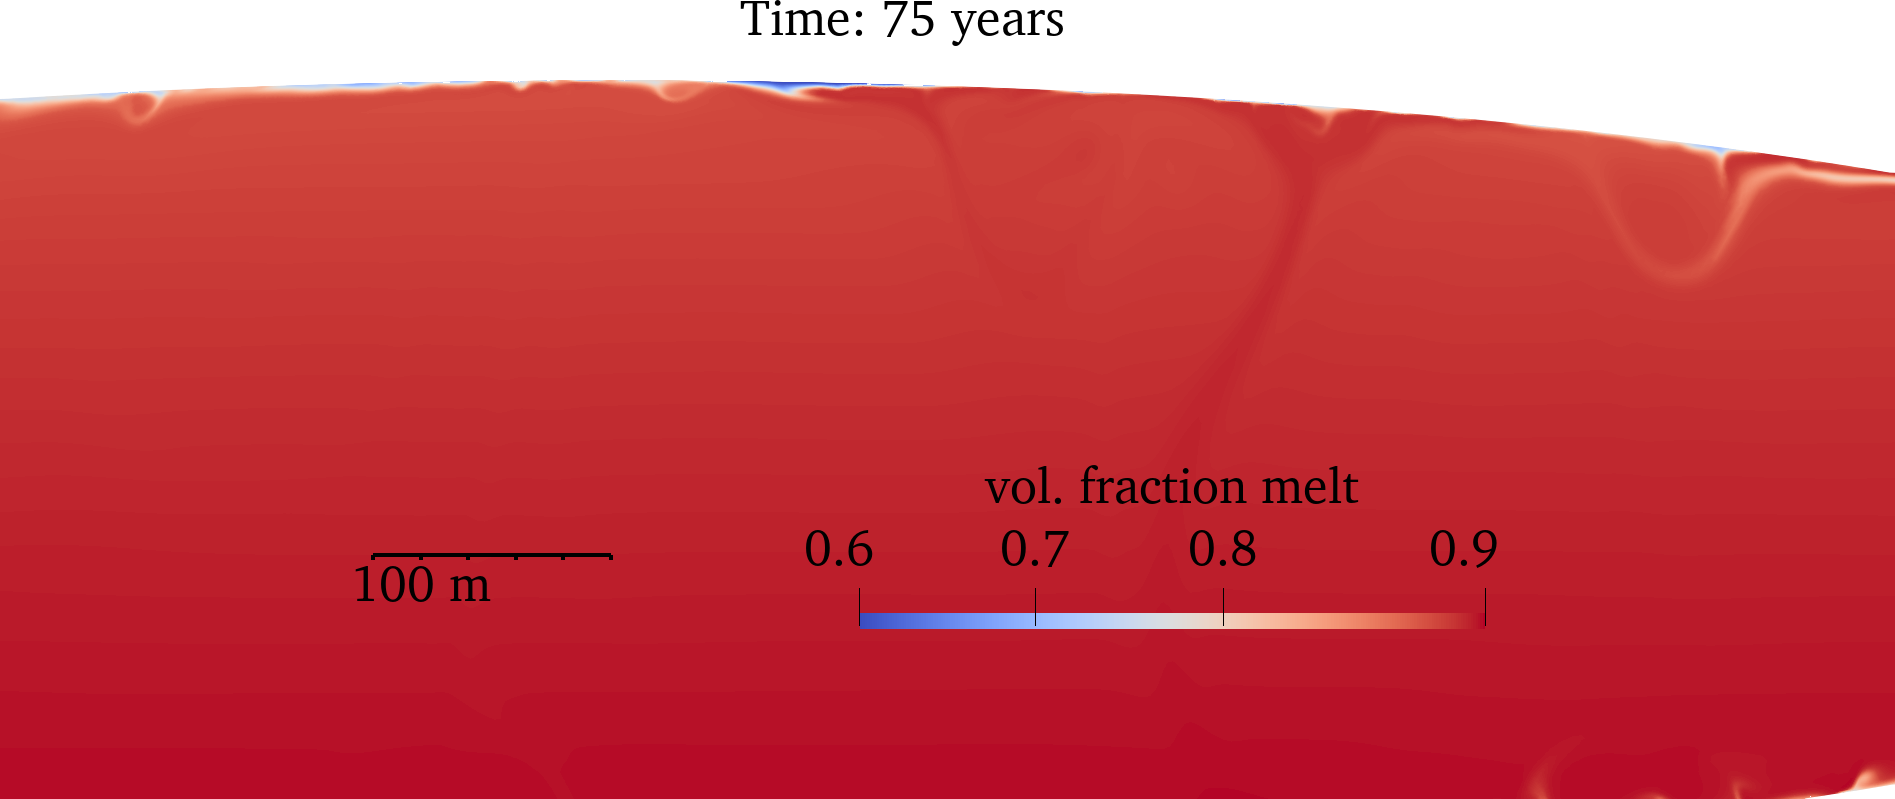
\includegraphics[width=0.86\linewidth]{img/chapter4/vf_l_75.png}};
		\node[anchor=north east, xshift=-0pt, yshift=-50pt] at (img1.north east) {\textbf{(a)}};
	\end{tikzpicture}
	\begin{tikzpicture}
		\node[inner sep=0pt] (img1) at (0,0)    {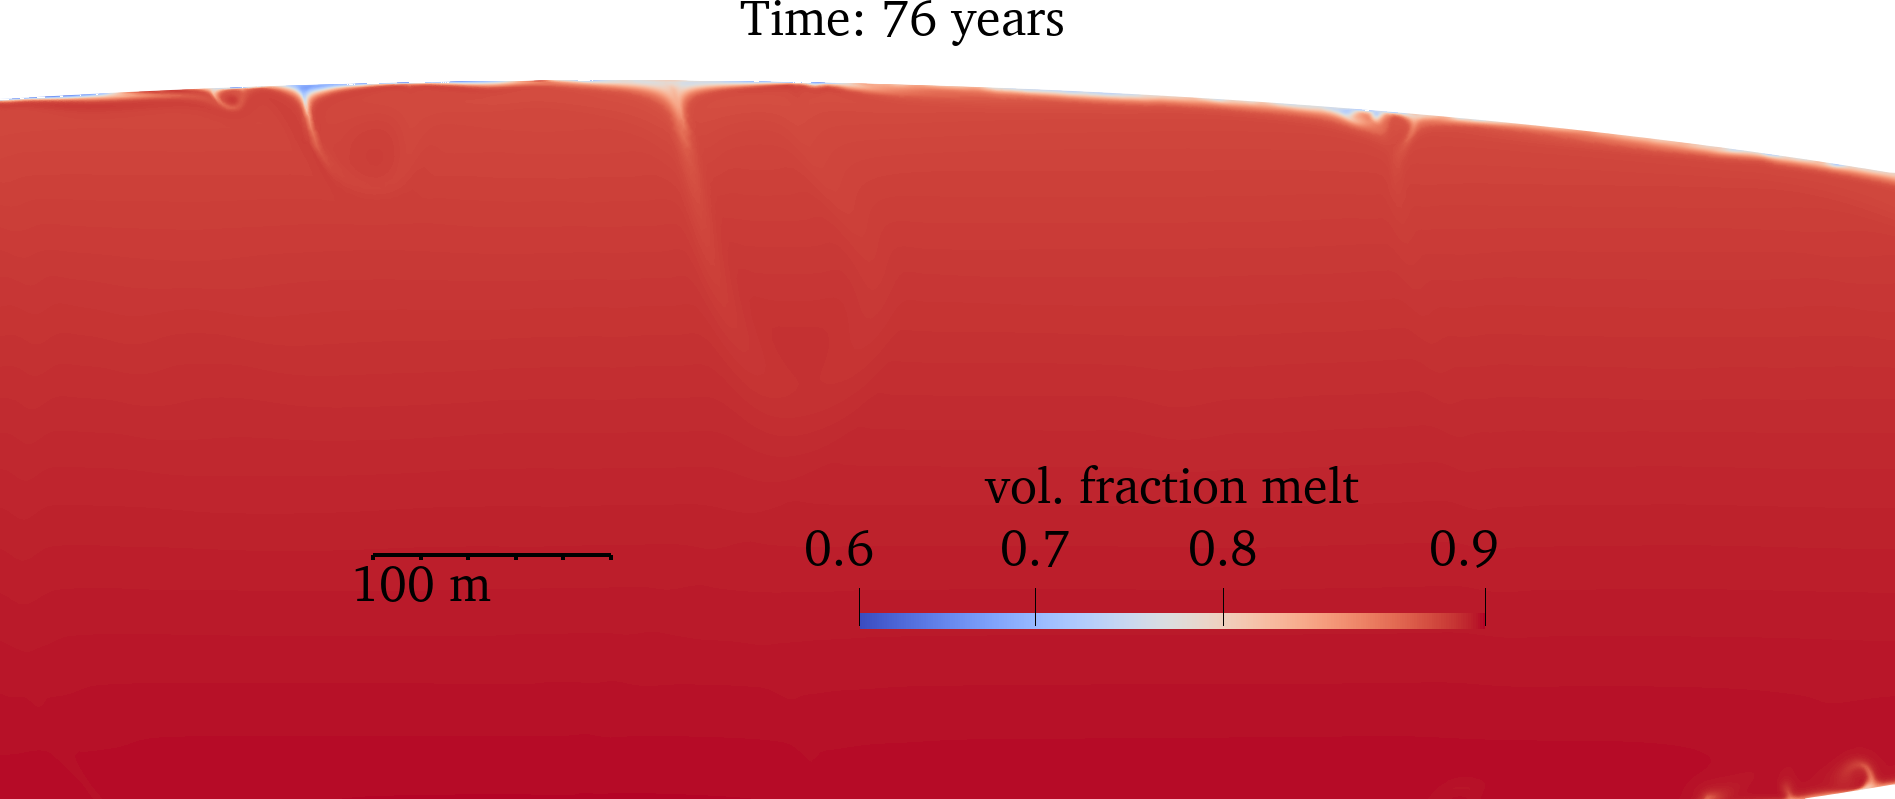
\includegraphics[width=0.86\linewidth]{img/chapter4/vf_l_76.png}};
		\node[anchor=north east, xshift=-0pt, yshift=-1pt] at (img1.north east) {\textbf{(b)}};
	\end{tikzpicture}	
	\caption{Snapshots of a zoomed-in area on the base simulation showing the evolution of the volume fraction of melt close to the boundary during 4 years. It can be seen that the thin crystallization front is quickly re-mobilized and reabsorbed.}
	\label{fig:73_76}
\end{figure}


% \begin{figure}
	% 	\centering
	% 	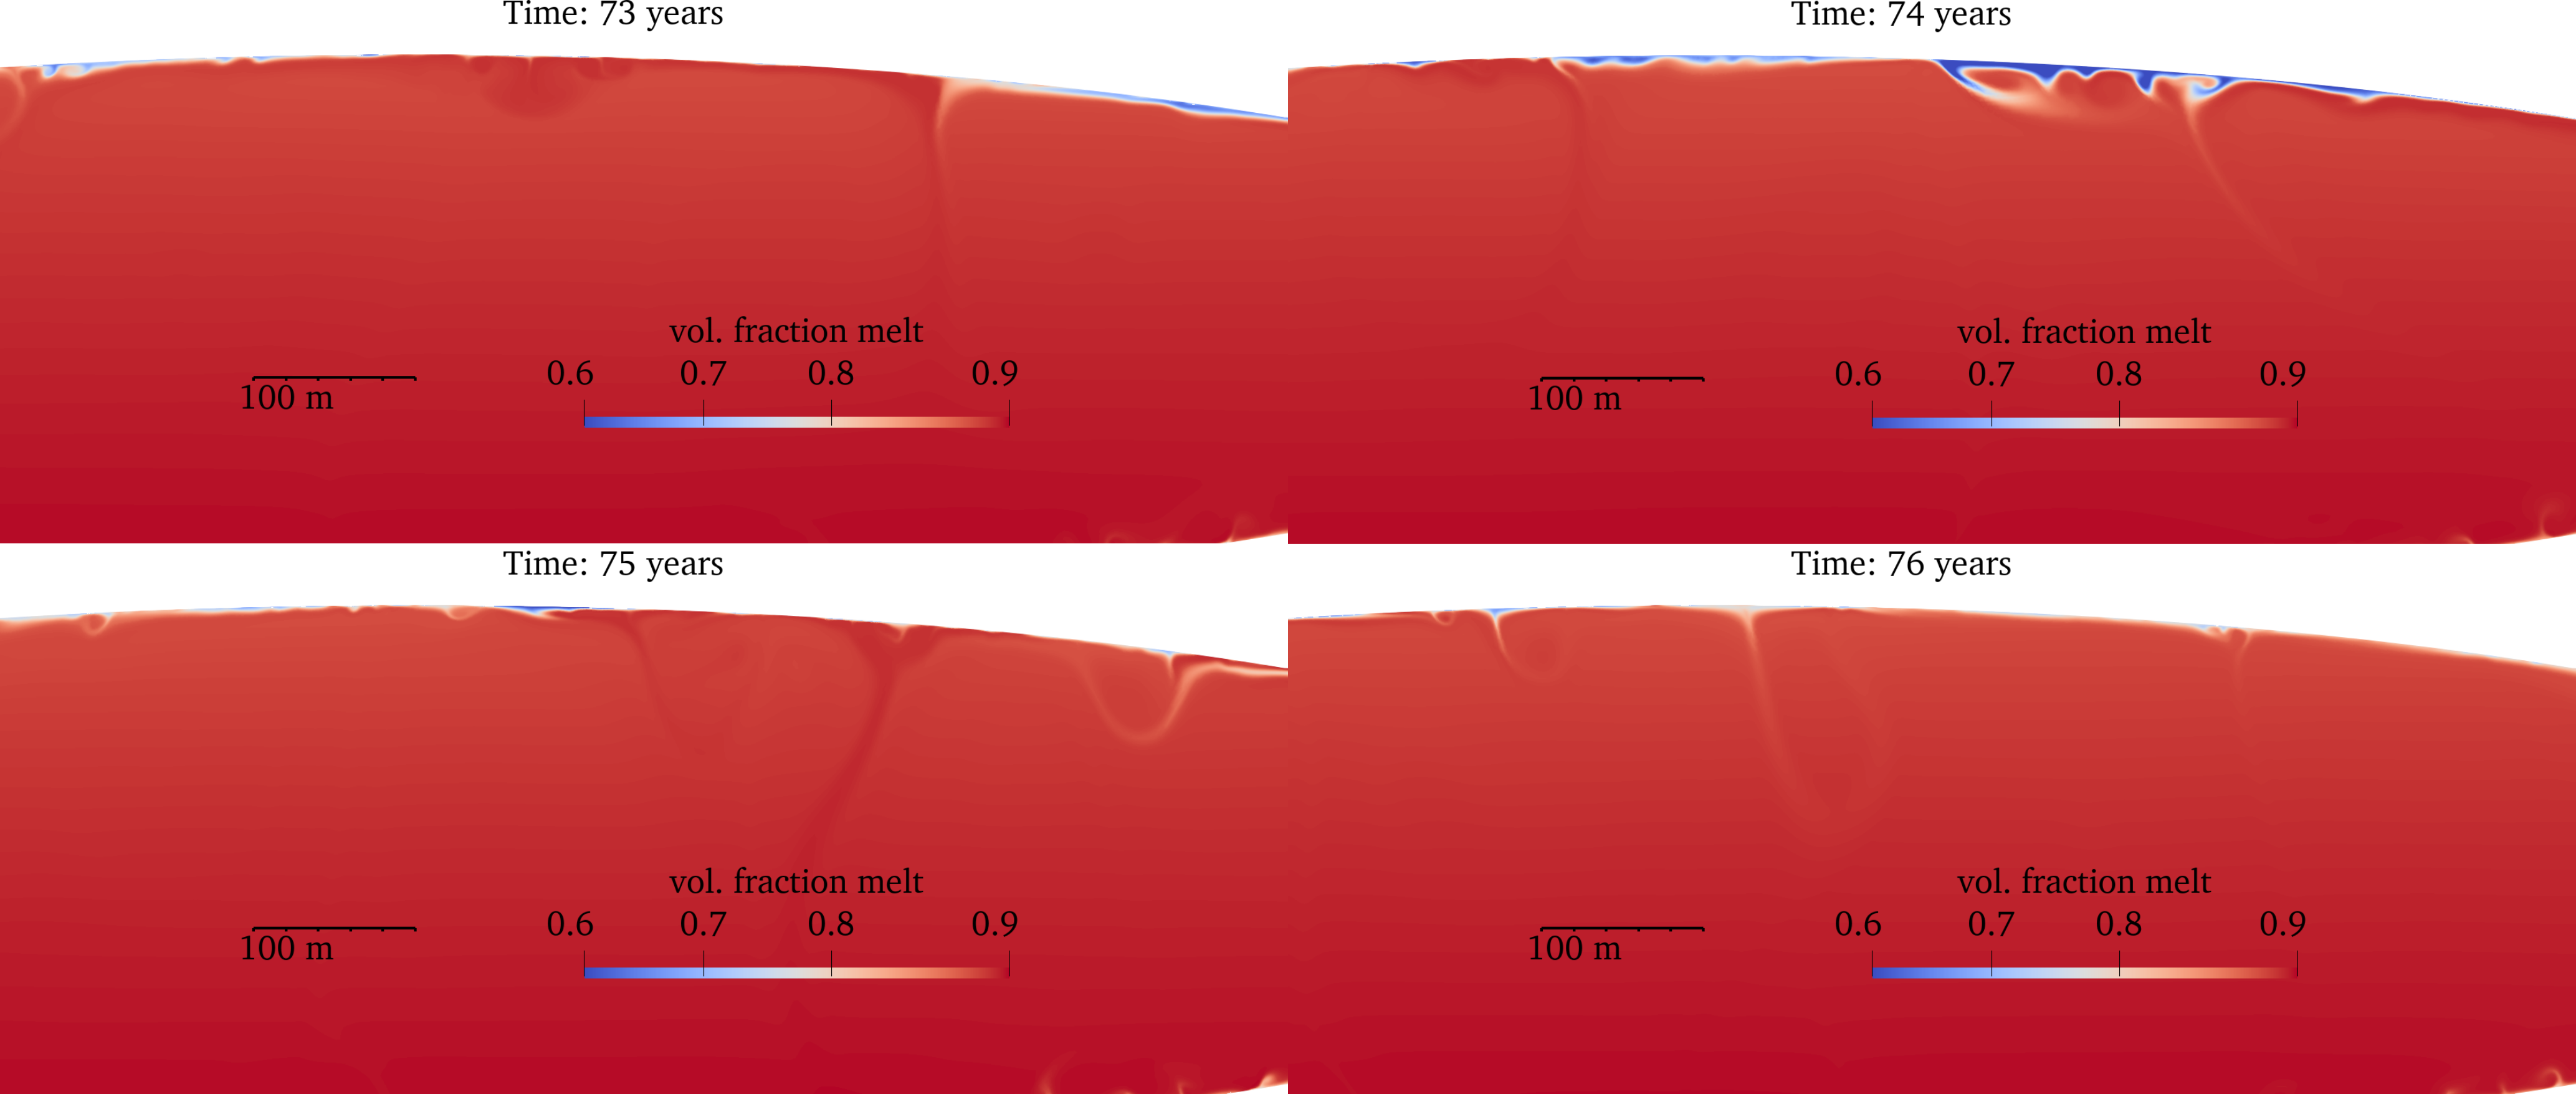
\includegraphics[width=1\linewidth]{img/chapter4/73_76.png}
	% 	\caption{Comparative plot of the time series of the integrated temperature for the three simulated sizes: small (blue), medium (green) and large (red).}
	% 	\label{fig:73_76}
	% \end{figure}